% ---------------------------------------------------
% TSP 2016 Conference Template
% ---------------------------------------------------


\documentclass[conference,a4paper,twocolumn]{IEEEtran}

\IEEEoverridecommandlockouts


% *** GRAPHICS RELATED PACKAGES ***
%
\ifCLASSINFOpdf
\else
\fi


  \usepackage{tipa}
  \usepackage[pdftex]{graphicx}
	\usepackage{epsfig}
	\usepackage{epstopdf}


% *** MATH PACKAGES ***
%
\usepackage[cmex10]{amsmath}


% *** SUBFIGURE PACKAGES ***
\usepackage{subfigure}

\hyphenation{op-tical net-works semi-conduc-tor}

% *** CUSTOME (added by Alexander Senov) PACKAGES ***
%\usepackage[utf8x]{inputenc} % указывает кодировку документа
%\usepackage[T2A]{fontenc} % указывает внутреннюю кодировку TeX 
\usepackage[english]{babel} % указывает язык документа
%\usepackage{lmodern}
%\usepackage{gentium}
%\renewcommand*\rmdefault{phv}
\usepackage{color} % для цветного текста

\usepackage{lipsum} % for dummy text

\newcommand{\convnet}{ConvNet~} % я не знаю как правильно называть сетку в тексте, вместо этого вставляю эту команду

\newcommand{\todo}[1]{\textcolor{red}{\textbf{[#1]}}} % чтобы в глаза бросалось
% ---------------------------------------------------
% Begin of Document
% ---------------------------------------------------

\begin{document}

% ---------------------------------------------------
% Title
% ---------------------------------------------------

% Titles are generally capitalized except for words such as a, an, and, as,
% at, but, by, for, in, nor, of, on, or, the, to and up, which are usually
% not capitalized unless they are the first or last word of the title.
% Linebreaks \\ can be used within to get better formatting as desired.
% Do not put math or special symbols in the title.


\title{Arabic Manuscript Author Verification Using\\ 
Deep Convolutional Networks}

% ---------------------------------------------------
% Authors, Affiliation, and Acknowledgment
% ---------------------------------------------------



% conference papers do not typically use \thanks and this command
% is locked out in conference mode. If really needed, such as for
% the acknowledgment of grants, issue a \IEEEoverridecommandlockouts
% after \documentclass

% for over three affiliations, or if they all won't fit within the width
% of the page, use this alternative format:
% 
\author{
\IEEEauthorblockN{
Andrei Boiarov\IEEEauthorrefmark{1},
Alexander Senov\IEEEauthorrefmark{2},
Alexander Knysh\IEEEauthorrefmark{3} and
Dmitry Shalymov\IEEEauthorrefmark{4}
}
\IEEEauthorblockA{
	\IEEEauthorrefmark{1}\IEEEauthorrefmark{2}\IEEEauthorrefmark{4}
	Faculty of Mathematics and Mechanics\\
	Saint Petersburg State University\\
	Saint Petersburg, Russia\\
	Email: 
		\IEEEauthorrefmark{1}a.boiarov@spbu.ru, 
		\IEEEauthorrefmark{2}alexander.senov@gmail.com, 
		\IEEEauthorrefmark{4}dmitry.shalymov@gmail.com
}
\IEEEauthorblockA{
\IEEEauthorrefmark{3}Department of Near Eastern Studies\\
University of Michigan\\
St. Petersburg State University Laboratory of Analysis and Modeling of Social Processes\\
%Ann Arbor, Michigan 48104-1608, USA\\
Ann Arbor, Michigan, USA\\
Email: alknysh@umich.edu}
\thanks{This research is supported by Saint Petersburg State University grant 6.37.181.2014. The authors express their deep gratitude to Mrs. Evyn Kropf of the Hatcher Graduate Library who kindly facilitated access to the University of Michigan library resources.}
}

% use for special paper notices
%\IEEEspecialpapernotice{(Invited Paper)}




% make the title area
\maketitle


% ---------------------------------------------------
% Abstract
% ---------------------------------------------------

% As a general rule, do not put math, special symbols or citations
% in the abstract
\begin{abstract}
\lipsum[5]
\end{abstract}

% no keywords

% For peer review papers, you can put extra information on the cover
% page as needed:
% \ifCLASSOPTIONpeerreview
% \begin{center} \bfseries EDICS Category: 3-BBND \end{center}
% \fi
%
% For peerreview papers, this IEEEtran command inserts a page break and
% creates the second title. It will be ignored for other modes.
\IEEEpeerreviewmaketitle

% ---------------------------------------------------
% Introduction
% ---------------------------------------------------

\section{Introduction}
\label{sec:introduction}
The present study was motivated by the recent discovery by Dr. Noah Gardiner of the holograph (autograph) copy of the third volume of al-Maqrizi's famous “Description of Egypt” in the Library of the University of Michigan (Michigan Islamic MS 605) \cite{Noah}. The full title of the manuscript is "al-Mawa'iz wa-al-i'tibar fi dhikr al-khitat wa-al-athar" ("The Book of Admonitions and Lessons in the Catalogue of Territorial Divisions and Historical Monuments"; usually cited simply as al-Khitat). The manuscript was copied well after 818 A.H. (1415 C.E.) and was finished shortly after 831 (1427) by the celebrated Egyptian historian Taqi al-Din Ahmad Ibn 'Ali al-Maqrizi (d. 845/1442). It is the only known Maqrizi holograph (autograph) in the Americas. A number of elements in the codex, including the apparent age of the paper, lacunae in the text where the dates of certain events had not been filled in, and a number of marginal addenda and sewn-in inserts containing text found in the printed editions, led Dr. Gardiner to suspect that it might be a draft copy of the work. He visually collated the predominant hand of the codex and the inserts with some published images of al-Maqrizi’s hand and felt that a match was highly likely. He then sent images of the codex to Prof. Frederic Bauden of the University of Liege, the author of numerous articles on al-Maqrizi autographs. Prof. Bauden confirmed that the codex was indeed copied by al-Maqrizi himself, and was thus a holograph (autograph). He identified it as the fair copy (the author’s final version) of the third volume of al-Khitat, and thus the only fair copy of any volume of al-Khitat to have been found.

Given the importance of this discovery for the history of science (al-Maqrizi's Khitat is one of the earliest descriptions of the topography of Cairo and ancient Egyptian monuments in its environs as well as Alexandria), a cross-disciplinary team of researchers affiliated with the St. Petersburg State University (Laboratory of Analysis and Modeling of Social Processes) decided to verify Dr. Gardiner’s and Prof. Bauden’s findings by using method based on deep convolutional networks.

Previously used methods for author verification of arabic manuscript and for related fields were focused on developing of various types of features that can be obtained from a manuscript picture \cite{MBulacu}, \cite{DFecker}. In this paper we present a novel approach based on learning of deep hierarchical structure of features from the row image. This method belongs to the class of deep learning algorithms \cite{DL} and uses convolutional network \cite{CNN} for feature extraction and prediction. Deep convolution networks since 2012 year \cite{Alexnet} became the state of the art in many areas of computer vision: objects recognition, face identification, optical character recognition, object detection etc \cite{DL}.

The paper is organized as follows. In the next section is given a description of data set used in experiments. Section III contains presentation of our methodology of extracting patches from image, training deep convolution networks and making decision of manuscript author. In section IV we present results of our experiments. At the end, conclusion is given.  
%\pagebreak
	

\begin{figure*}[!t]
	\center
  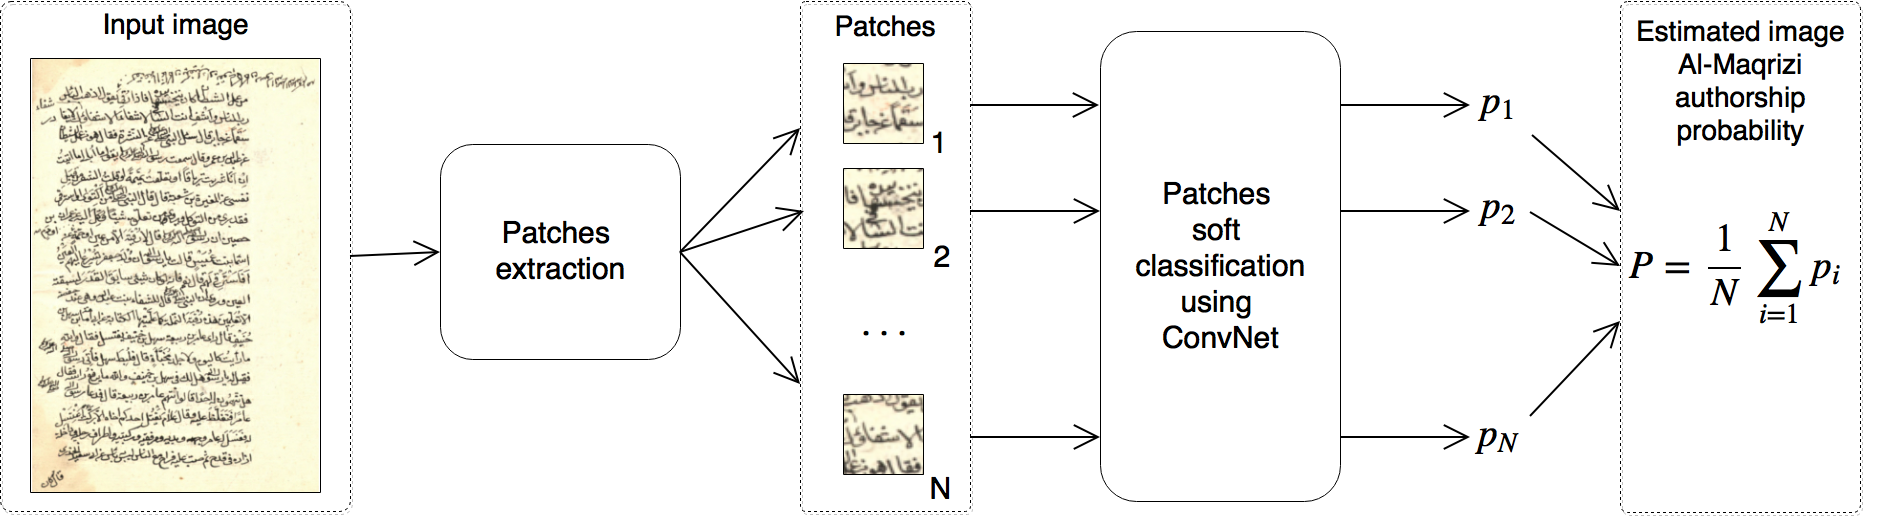
\includegraphics[width=\textwidth]{figures/Al-Maqrizi_classification_pipeline.png}
  \caption{Al-Maqrizi authorship soft classification pipeline}
  \label{fig:pipeline}
\end{figure*}	
	
\section{Data Set}
\label{sec:the_data}

Solving of the problem of al-Maqrizi authorship verification requires training and validation data sets. As a one unique data element we consider single page of manuscript. Data set composes of a set of consistent parts from manuscripts of two kinds:
\begin{itemize}
	\item Two sets of verified al-Maqrizi's holographs from codex of Prof. Bauden is taken as a positive examples.
	\item Eight manuscripts not written by al-Maqrizi's hand from the University of Michigan Hatcher Library (Special Collections) are considered as a negative examples. This manuscripts are selected in such way that the date and place of writing each of them is close to al-Maqrizi's Khitat: 14th and 15th centuries, Egypt and Syria.
\end{itemize}
For robustness of learning process obtained data is divided into training and validation sets:
\begin{itemize}
	\item Training set: 1 al-Maqrizi's manuscript consisting of 26 pages and 5 not al-Maqrizi's manuscripts each of which consists of 7 pages.
	\item Validation set: 1 al-Maqrizi's manuscript consisting of 14 pages and 3 not al-Maqrizi's manuscripts each of which consists of 7 pages. Authors of this 3 manuscripts differ from authors of 5 negative examples in training set.   
\end{itemize}

It is important to note that we split our data set by the factor of a manuscript author. Thus when algorithm is learning on training set, it can not see authors in validation set. In that way we achieve robustness our method in terms of manuscripts because input of method is a whole manuscript. Number of not al-Maqrizi's documents is chosen in such way that training and validation set is nearly balanced.

Main interest of this paper is author verification of al-Khitat manuscript consisting of 32 pages.


%\pagebreak

\section{Method}
\label{sec:the_method}

We consider author verification problem as a binary classification problem: Al-Maqrizi class denoted as $1$ and non-Al-Maqrizi class denoted as $0$. In this context our goal is to build a classification pipeline able predict the probability (\textit{soft} classification) that given image belongs to the $1$ (Al-Maqrizi) class. The entire Al-Maqrizi authorship classification pipeline illustrated at figure~\ref{fig:pipeline} consists of the following steps:

\begin{enumerate}
	\item Image preprocessing.
	\item Extracting patches from candidate image.
	\item Patches soft classification using \convnet.
	\item Averaging predicted patches probabilities to produce overall candidate image Al-Maqrizi authorship probability.
\end{enumerate}



Each of this steps are thoroughly described in the following sections.	

%The heart of our method is a \convnet patches classifier. We use ground-truth labelled patches extracted from images described in section~\ref{sec:the_data} as a training set for \convnet. [SOME DEFERRABLES FOR \convnet HERE].

\todo{Describe image preprocessing}

\subsection{Patches extraction}
The patches extraction method generates a set of sub-images called patches from given image. The basic idea is that patch should represent small but yet meaningful part of image for the main purpose - authorship verification. We use two alternative methods for patches extraction described in following subsections.

\subsubsection{Sliding window based method}
This method splits given image by a grid of fixed cell size. Each cell further used as a patch. Figure~\ref{fig:patches_example_sliding_window} \todo{add figure} illustrates the idea. 

\subsubsection{Connected components based method}
This method uses following routine for patches extraction

\begin{enumerate}
	\item Input image binarization using Otsu's filter \todo{reference to Otsu filter paper}.
	\item Connected components extraction from binarized image using algorithm from \todo{reference to connected components paper}.
c	\item Too small, too big and too stretched connected components filtering using several empirical rules \todo{specific rules description}.
	\item Outlier connected components filtering using DBSCAN \todo{reference to DBSCAN paper} clustering algorithm.
	\item Using remaining connected components bounding boxes as patches.
\end{enumerate}

Example of connected components based patches show on figure~\ref{fig:patches_example_connected components} \todo{add figure}. 

It could be seen, that connected components based patches usually consist of one or few letters thus providing high robustness for different image scale and size in contrast to fixed-size sliding window patches. However, fixed-sliding patches contain much more information: several symbols from several lines, - a very important feature for the authorship verification.



\todo{Fill this section}


\section{Results and Discussion}


\todo{Fill this section}

\section{Conclusion}

The join research on al-Maqrizi’s “Description of Egypt” undertaken by a historian-philologist and three mathematicians from St. Petersburg State University is a unique experiment in working across disciplinary boundaries to achieve a common goal. Its results bode well for the future by opening new horizons for scholars of “Oriental” manuscripts who often desperately lack resources (other than their own eyes and intuition) to verify the provenance and authorship of the manuscript material they are working with. Given the propensity of Muslim scribes and later writers to attribute manuscripts to important luminaries of the past (such as, e.g., al-Ghazali, d. 505/1111; Ibn al-ʿArabi, d. 638/1240, and others), the new methods of analyzing and verifying handwritten texts, which have been designed and tested by St. Petersburg mathematicians, are bound to become an important tool for their colleagues in the humanities and social sciences.

% ---------------------------------------------------
% References
% ---------------------------------------------------

% can use a bibliography generated by BibTeX as a .bbl file
% BibTeX documentation can be easily obtained at:
% http://www.ctan.org/tex-archive/biblio/bibtex/contrib/doc/
% The IEEEtran BibTeX style support page is at:
% http://www.michaelshell.org/tex/ieeetran/bibtex/
%\bibliographystyle{IEEEtran}
% argument is your BibTeX string definitions and bibliography database(s)
%\bibliography{IEEEabrv,../bib/paper}
%
% <OR> manually copy in the resultant .bbl file
% set second argument of \begin to the number of references
% (used to reserve space for the reference number labels box)

\begin{thebibliography}{99}

\bibitem{Noah} N.~Gardiner, F.~Bauden, \lq\lq A Recently Discovered Holograph Fair Copy of al-Maqrīzī’s al-Mawāʿiẓ wa-al-iʿtibār fī dhikr al-khiṭaṭ wa-al-āthār (Michigan Islamic MS 605),\rq\rq~in~\emph{Journal of Islamic Manuscripts}, vol.~2, E.~J.~Brill, Leiden and Boston, 2011, pp.~123--131.

\bibitem{MBulacu} M.~Bulacu, L.~Schomaker, A.~Brink \lq\lq Text-independent writer identification and verification on offline arabic handwriting,\rq\rq~in~\emph{Proc. 9th International Conference on Document Analysis and Recognition, ICDAR}, Curitiba, 2007, pp.~769--773.

\bibitem{DFecker} D.~Fecker, A.~Asi, W.~Pantke, V.~Märgner, J.~El-Sana, T.~Fingscheidt \lq\lq Document Writer Analysis with Rejection for Historical Arabic Manuscripts,\rq\rq~in~\emph{Proc. 14th nternational Conference on Frontiers in Handwriting Recognition, ICFHR}, Crete, 2014, pp.~743--748.

\bibitem{DL} Y.~Lecun, Y.~Bengio, G.~Hinton, \lq\lq Deep learning,\rq\rq~\emph{Nature}, no.~521, pp.~436--444, May.~2015.

\bibitem{CNN} Y.~Lecun, L.~Bottou, Y.~Bengio, P.~Haffner, \lq\lq Gradient-based learning applied to document recognition,\rq\rq~in~\emph{Proc. of the IEEE}, 1998, pp.~2278--2324.

\bibitem{Alexnet} A.~Krizhevsky,I.~Sutskever, G.~Hinton, \lq\lq ImageNet Classification with Deep Convolutional Neural Networks,\rq\rq~in~\emph{Advances in Neural Information Processing Systems}, vol.~25, 2012, pp.~1097--1105.

\bibitem{Googlenet} C.~Szegedy, W.~Liu, Y.~Jia, P.~Sermanet, S.~Reed, D.~Anguelov, D.~Erhan, V.~Vanhoucke, A.~Rabinovich, \lq\lq Going deeper with convolutions,\rq\rq~in~\emph{Proc. of the IEEE Conference on Computer Vision and Pattern Recognition}, Boston, 2015, pp.~1--9.

\bibitem{GranVolk} O.~Granichin, V.~Volkovich, D.~Toledano-Kitai, \emph{Randomized Algorithms in Automatic Control and Data Mining}. Springer-Verlag: Heidelberg, New York, Dordrecht, London, 2015, 251~p.

\end{thebibliography}

% ---------------------------------------------------
% End of Document
% ---------------------------------------------------

% that's all folks
\end{document}


